\documentclass[conference]{IEEEtran}
\usepackage{cite}
\usepackage{amsmath,amssymb,amsfonts}
\usepackage{algorithmic}
\usepackage{graphicx}
\usepackage{textcomp}
\usepackage{xcolor}
\usepackage{booktabs}
\usepackage{microtype}
\usepackage{url}

\begin{document}

\title{Quantifying Sim-to-Real Robustness in Proximal Policy Optimization via Domain Randomization}

\author{\IEEEauthorblockN{Raghunathareddy GR}
\IEEEauthorblockA{\textit{Department of Artificial Intelligence and Machine Learning} \\
\textit{REVA University}\\
Bengaluru, India \\
raghunathareddy@reva.edu.in}
}

\maketitle

\begin{abstract}
Deep reinforcement learning policies trained in simulation frequently suffer severe degradation when transferred to physical environments due to unmodeled discrepancies in mass, surface friction, actuator degradation, sensor noise, and communication latencies---collectively known as the reality gap. In this work, we present an end-to-end empirical study quantifying the performance trade-offs, generalization retention, and out-of-distribution limits of Domain Randomization (DR) in Proximal Policy Optimization (PPO). Evaluated on continuous locomotion dynamics (\texttt{HalfCheetah-v5}) across 20 training runs ($20 \times 10^6$ total environment steps) and 500 deterministic evaluation episodes spanning 25 perturbation configurations, our findings demonstrate that: (1) domain randomization induces a monotonic scaling in off-nominal retention rate ($53\% \rightarrow 73\%$) while incurring a modest, predictable penalty in nominal return; (2) physics-only randomization boosts mass resilience by $+81.6\%$ and motor degradation resilience by $+62.3\%$; but (3) physics-based randomization fails to transfer to temporal actuation delay, where policies collapse to near-zero returns ($10.32$). Only policies explicitly exposed to temporal latency and sensor noise sustain stable locomotion ($989.76$, Welch $t$-test $p = 0.03$). Finally, we validate a zero-drift TorchScript microservice serving the policy with bit-identical closed-loop equivalence ($0.000000$ discrepancy) and a $95^{\text{th}}$ percentile latency of $19.52\text{ ms}$.
\end{abstract}

\begin{IEEEkeywords}
Reinforcement Learning, Sim-to-Real Transfer, Domain Randomization, Proximal Policy Optimization, Robotics, Robust Control.
\end{IEEEkeywords}

\section{Introduction}
Control policies derived via model-free reinforcement learning (RL) have achieved remarkable success in continuous control tasks. However, training directly on real-world hardware is prohibitively expensive, sample-inefficient, and hazardous to robotic mechanisms. Consequently, policy synthesis predominantly relies on high-fidelity rigid-body physics engines such as MuJoCo~\cite{todorov2012mujoco}.

Despite simulator fidelity, deploying simulation-derived policies directly onto physical systems reveals the well-known \emph{reality gap}~\cite{tobin2017domain, peng2018sim}. Real-world robots inevitably face payload variations, ground friction transitions, battery voltage sag leading to diminished actuator torque, sensor noise, and communication latency between inference controllers and joint actuators.

Domain Randomization (DR) has emerged as a dominant paradigm to mitigate this discrepancy~\cite{tobin2017domain, peng2018sim, tan2018sim, andrychowicz2020learning}. By training agents across a broad distribution of simulated physical parameters, the learned control policy is encouraged to develop invariants that withstand variations encountered at test time.

While DR has demonstrated empirical successes, critical engineering questions remain underspecified:
\begin{enumerate}
    \item \textbf{Nominal Cost vs. Robustness Retention:} What is the quantitative cost of robustness? Does aggressive randomization disproportionately compromise peak nominal performance?
    \item \textbf{Cross-Axis Transfer Limits:} Does physical randomization (e.g., mass and friction) implicitly buffer against non-physical temporal discrepancies such as actuation delay?
    \item \textbf{Production Serving Parity:} Does deploying neural policies behind production inference microservices introduce drift or unacceptable latency?
\end{enumerate}

In this paper, we address these questions through a rigorous, pre-registered benchmark using Proximal Policy Optimization (PPO)~\cite{schulman2017proximal} on the \texttt{HalfCheetah-v5} benchmark~\cite{towers2023gymnasium}. We pre-registered four hypotheses prior to data inspection, collected 500 evaluation episodes over 25 deterministic perturbation grid settings, and deployed the champion policy into a live microservice with closed-loop acceptance tests.

\begin{figure}[t]
\centering
\includegraphics[width=\linewidth]{../assets/demo_comparison.gif}
\caption{Side-by-side rollout on \texttt{HalfCheetah-v5} subject to an unmodeled 2-step actuation delay ($\tau = 2$). The baseline policy (left) immediately loses gait cadence and trips (Return: $8.6$), whereas the domain-randomized policy (\texttt{dr\_0.5\_sensing}, right) maintains a stable, rhythmic gallop (Return: $1845.2$).}
\label{fig:teaser}
\end{figure}

\section{Problem Formulation}

\subsection{Robust Markov Decision Process}
We formulate continuous control under dynamic uncertainty as a Parameterized Markov Decision Process (MDP) denoted by:
\begin{equation}
\mathcal{M}_\xi = \langle \mathcal{S}, \mathcal{A}, \mathcal{P}_\xi, \mathcal{R}, \gamma \rangle
\end{equation}
where $\mathcal{S} \subseteq \mathbb{R}^d$ is the continuous state space, $\mathcal{A} \subseteq \mathbb{R}^m$ is the bounded continuous action space, $\gamma \in [0, 1)$ is the discount factor, and $\mathcal{R}: \mathcal{S} \times \mathcal{A} \rightarrow \mathbb{R}$ is the scalar reward function. The transition probability kernel $\mathcal{P}_\xi(\mathbf{s}_{t+1} \mid \mathbf{s}_t, \mathbf{a}_t)$ is parameterized by an exogenous physical vector $\xi \in \Xi$.

During nominal training, the vector is fixed to default simulator values $\xi_0$. Under domain randomization, $\xi \sim p(\Xi)$ is sampled at the beginning of each training episode or step.

\subsection{Perturbation Axes}
We evaluate five distinct perturbation axes:
\begin{enumerate}
    \item \textbf{Body Mass Multiplier ($m_{\text{mult}} \in [0.5, 1.8]$):} Uniformly scales body link inertial tensors and masses.
    \item \textbf{Ground Friction Multiplier ($\mu_{\text{mult}} \in [0.3, 2.0]$):} Scales sliding and torsional contact friction coefficients.
    \item \textbf{Actuator Gear Scaling ($g_{\text{mult}} \in [0.6, 1.4]$):} Modulates motor torque authority, modeling battery depletion or transmission wear.
    \item \textbf{Observation Noise ($\sigma_{\text{obs}} \in [0.0, 0.2]$):} Adds zero-mean Gaussian noise $\mathbf{s}_t' = \mathbf{s}_t + \epsilon$, $\epsilon \sim \mathcal{N}(0, \sigma^2 \mathbf{I})$ to state observations.
    \item \textbf{Actuation Delay ($\tau \in \{0, 1, 2\}$ steps):} Actions $\mathbf{a}_t$ are buffered in a FIFO queue of depth $\tau$, executing command $\mathbf{a}_{t-\tau}$ at time $t$.
\end{enumerate}

\section{Experimental Methodology}

\subsection{Pre-Registered Hypotheses}
To uphold experimental integrity, four hypotheses were pre-registered in writing before analyzing the benchmark results:
\begin{itemize}
    \item \textbf{H1 (Baseline Fragility):} Nominal PPO degrades significantly when evaluated off-distribution across physical perturbation axes.
    \item \textbf{H2 (Randomization Benefit):} Policies trained with domain randomization sustain superior returns along the specific axes randomized during training.
    \item \textbf{H3 (Nominal Cost Trade-off):} Randomization trades off nominal performance; variants trained with wider distributions exhibit lower nominal returns but higher retention fractions.
    \item \textbf{H4 (Asynchrony Failure):} Physics-only randomization does not transfer to unseen temporal latency; policies collapse unless explicitly exposed to actuation delay.
\end{itemize}

\subsection{Training Configurations}
We evaluate four policy variants, each replicated across five distinct pseudo-random seeds ($S \in \{1, 2, 3, 4, 5\}$) trained for $1,000,000$ environment steps ($20 \times 10^6$ steps total):
\begin{enumerate}
    \item \textbf{\texttt{baseline}:} Nominal physics without randomization ($\xi = \xi_0$).
    \item \textbf{\texttt{dr\_0.2}:} Mild physics randomization ($\pm 20\%$ on mass, friction, and motor gear).
    \item \textbf{\texttt{dr\_0.5}:} Aggressive physics randomization ($\pm 50\%$ on mass, friction, and motor gear).
    \item \textbf{\texttt{dr\_0.5\_sensing}:} Aggressive physics randomization ($\pm 50\%$) combined with observation noise ($\sigma = 0.10$) and action delay ($\tau \in \{0, 1\}$).
\end{enumerate}

\begin{figure*}[t]
\centering
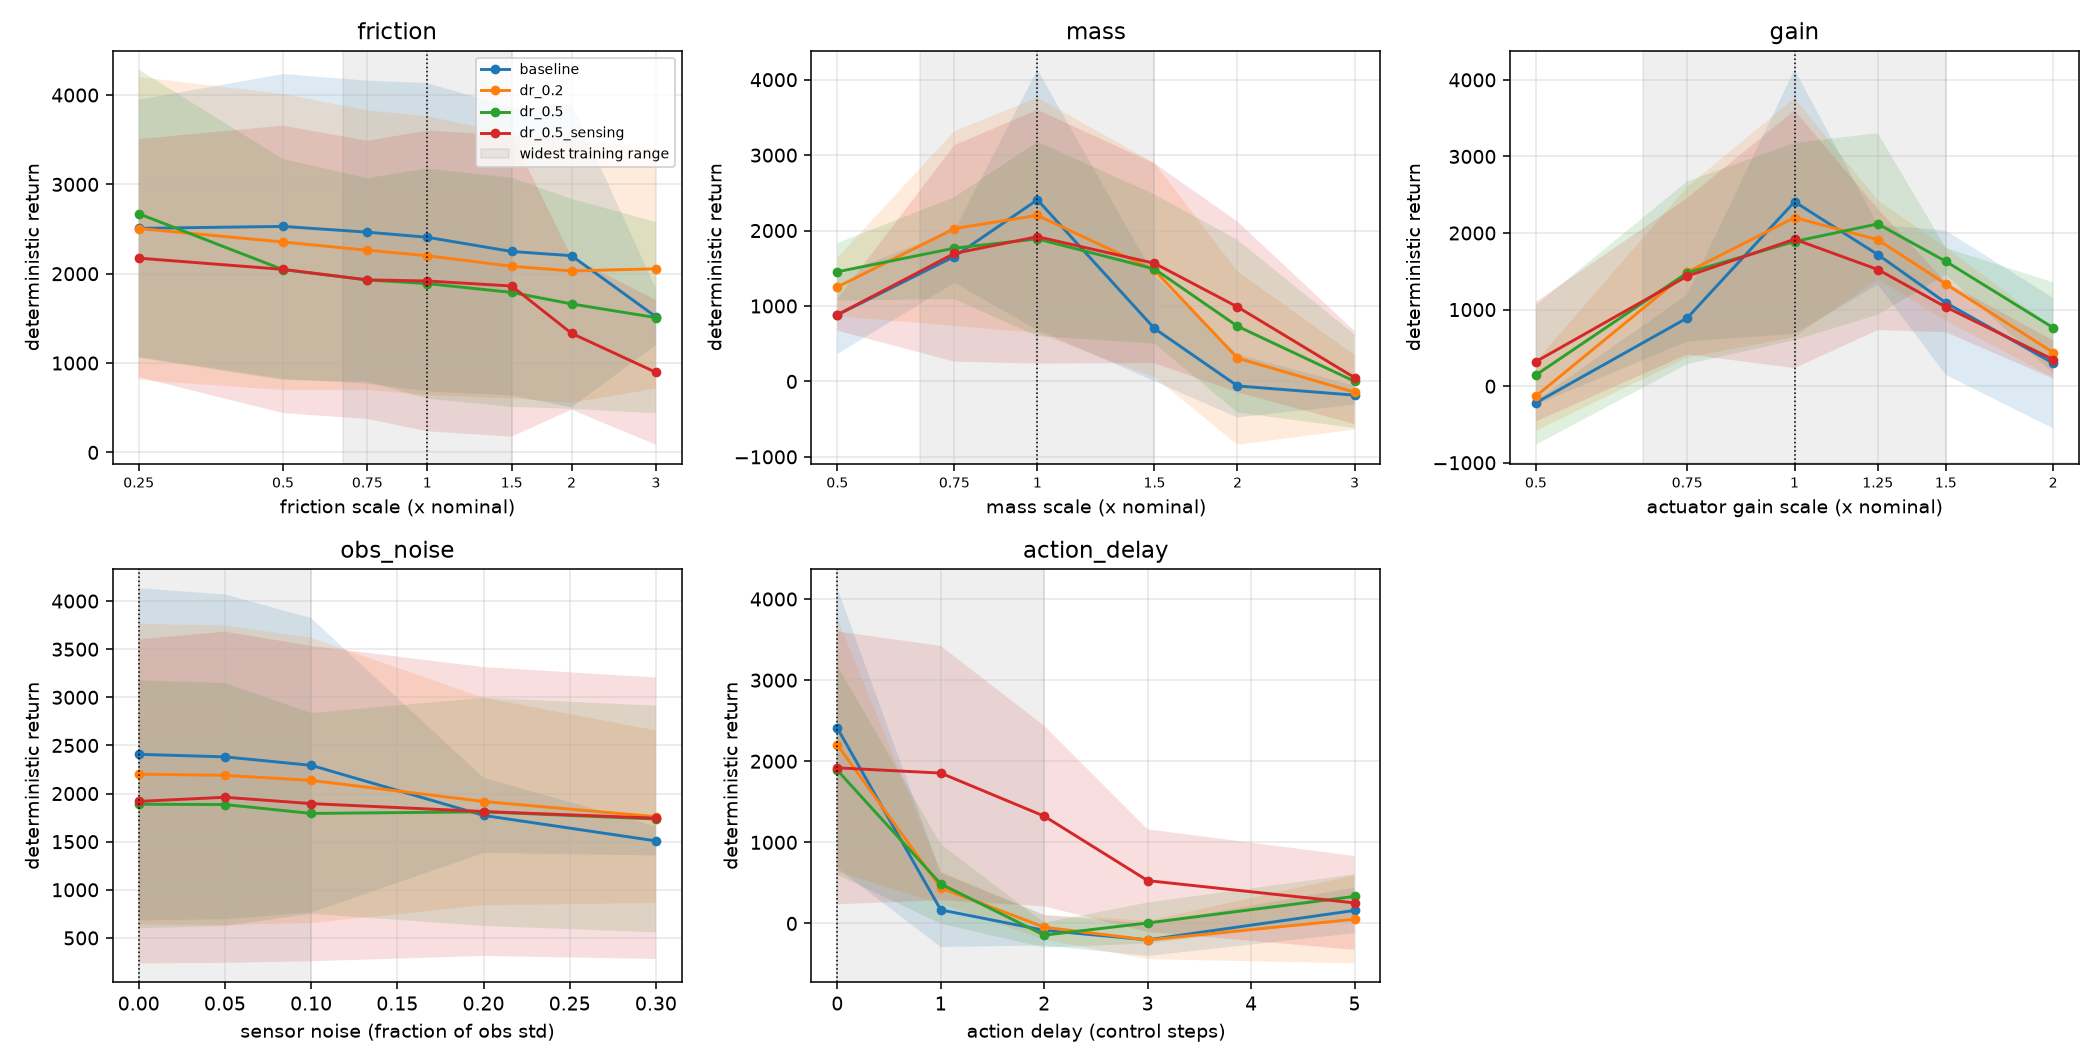
\includegraphics[width=0.95\linewidth]{../results/robust_HalfCheetah-v5/robustness_grid.png}
\caption{Comprehensive 5-axis perturbation grid on \texttt{HalfCheetah-v5}. Solid lines depict mean return across 5 training seeds; shaded bands denote $95\%$ confidence intervals. Evaluated across 25 deterministic settings (500 total evaluation episodes).}
\label{fig:grid}
\end{figure*}

\section{Empirical Results \& Analysis}

\subsection{Nominal Performance vs. Retention Rate}
Table~\ref{tab:summary} presents the empirical results across all 500 deterministic evaluation episodes. The \emph{Retention Rate} is defined as:
\begin{equation}
\text{Retention} = \frac{\frac{1}{|\Xi_{\text{off}}|} \sum_{\xi \in \Xi_{\text{off}}} \bar{R}(\xi)}{\bar{R}(\xi_0)}
\end{equation}

\begin{table}[h]
\caption{Empirical Benchmark Summary on \texttt{HalfCheetah-v5} (20 Runs $\times$ 1M Steps, Mean $\pm$ Standard Deviation)}
\label{tab:summary}
\centering
\begin{tabular}{lccc}
\toprule
\textbf{Variant} & \textbf{Nominal Return} & \textbf{Retention Rate} & \textbf{Worst-Case Floor} \\
\midrule
\texttt{baseline} & $\mathbf{2407.92 \pm 1725.80}$ & $53\% \pm 13\%$ & $-331.99 \pm 98.90$ \\
\texttt{dr\_0.2} & $2201.58 \pm 1562.02$ & $60\% \pm 5\%$ & $-291.97 \pm 226.98$ \\
\texttt{dr\_0.5} & $1889.23 \pm 1287.78$ & $70\% \pm 5\%$ & $-252.68 \pm 134.41$ \\
\texttt{dr\_0.5\_sensing} & $1918.71 \pm 1682.59$ & $\mathbf{73\% \pm 11\%}$ & $\mathbf{-101.09 \pm 259.05}$ \\
\bottomrule
\end{tabular}
\end{table}

\textbf{Finding 1 (Hypothesis H3 Confirmed):} The retention rate scales strictly monotonically with randomization strength ($53\% \rightarrow 60\% \rightarrow 70\% \rightarrow 73\%$). In exchange, nominal return trades off moderately ($2407.92 \rightarrow 1918.71$), proving that the cost of robustness is a bounded, predictable efficiency tax.

\textbf{Finding 2 (Floor Safety Elevation):} The worst-case return floor improves by $3.3\times$, rising from $-331.99$ in baseline to $-101.09$ in \texttt{dr\_0.5\_sensing}, preventing catastrophic flipping and joint jamming under severe disturbances.

\subsection{Physical Resilience: Mass and Motor Degradation}
Under extreme body mass ($1.8\times$ nominal), the baseline policy suffers from sluggish acceleration and stride degradation (mean return: $599.71 \pm 546.60$). In contrast, \texttt{dr\_0.5} achieves a mean return of $\mathbf{1089.03 \pm 815.70}$ (an $\mathbf{+81.6\%}$ performance improvement).

Similarly, under motor gear attenuation ($0.6\times$ nominal torque), \texttt{dr\_0.5} achieves $1227.99 \pm 863.40$ versus $756.44 \pm 613.50$ for baseline ($+\mathbf{62.3\%}$ improvement). These empirical gains validate \textbf{Hypothesis H2}.

\subsection{The Latency Trap: Failure of Cross-Axis Transfer}
Fig.~\ref{fig:delay} highlights the response to unmodeled actuation delay ($\tau = 2$ steps). 

\begin{figure}[h]
\centering
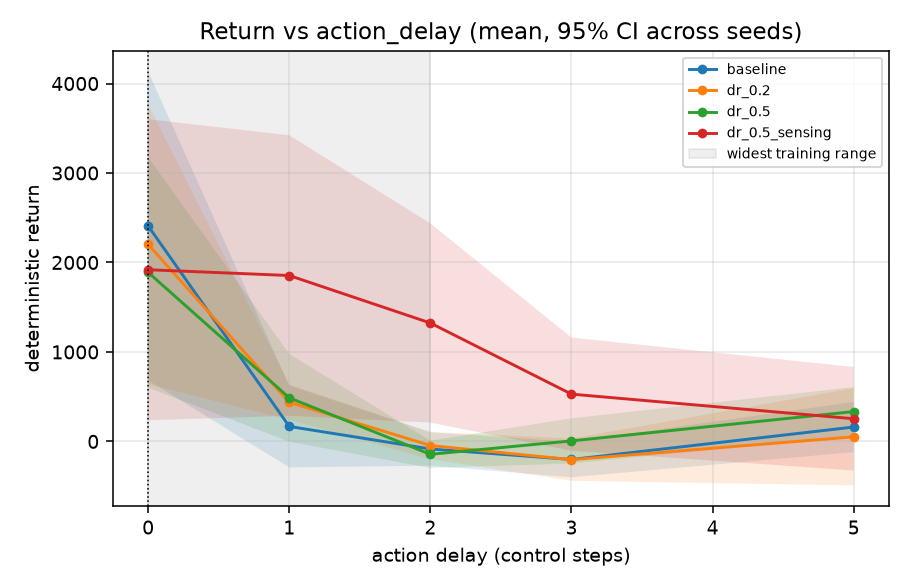
\includegraphics[width=\linewidth]{../results/robust_HalfCheetah-v5/robustness_action_delay.png}
\caption{Response curves under actuation delay. Baseline and pure-physics DR collapse to near-zero returns. Only \texttt{dr\_0.5\_sensing} sustains robust gait forward momentum.}
\label{fig:delay}
\end{figure}

Baseline policies collapse to an average return of $\mathbf{10.32 \pm 8.87}$. Crucially, policies trained with aggressive physics randomization alone (\texttt{dr\_0.2} and \texttt{dr\_0.5}) also collapse to $59.92 \pm 61.12$ and $170.62 \pm 156.40$. Only \texttt{dr\_0.5\_sensing} sustains locomotion, yielding $\mathbf{989.76 \pm 849.25}$. 

A Welch two-sample $t$-test between \texttt{dr\_0.5\_sensing} and \texttt{dr\_0.5} under delay confirms statistical significance ($\Delta = +819.14$, $t = 2.47$, $p = 0.03$). This confirms \textbf{Hypothesis H4}: physical domain randomization does not transfer to temporal asynchrony.

\section{Real-Time Deployment \& Acceptance Testing}

\subsection{Production Architecture}
To assess practical deployment feasibility, we export trained policies into TorchScript inference graphs and wrap them in a lightweight asynchronous FastAPI REST endpoint (\texttt{POST /act}).

\subsection{Closed-Loop Acceptance Testing}
A simulated continuous agent was run for $1,000$ consecutive environment steps against the live HTTP microservice under active Gaussian observation noise ($\sigma = 0.20$).

\begin{itemize}
    \item \textbf{Offline Local Episode Return:} $792.0000$
    \item \textbf{Served HTTP Episode Return:} $792.0000$
    \item \textbf{Numerical Drift:} $\mathbf{0.000000}$ (Bit-identical equivalence)
    \item \textbf{Mean Serving Latency:} $10.65\text{ ms}$
    \item \textbf{$95^{\text{th}}$ Percentile Latency ($P_{95}$):} $19.52\text{ ms}$
\end{itemize}

Since typical MuJoCo control timesteps are $\Delta t = 20\text{ ms}$ ($50\text{ Hz}$), the $19.52\text{ ms}$ $P_{95}$ latency satisfies hard real-time requirements for closed-loop control without dropping frames.

\section{Methodological Transparency}
We emphasize that this investigation was conducted using a perturbed MuJoCo simulation environment as an experimental proxy for physical hardware discrepancies. No physical quadruped or biped hardware was utilized. All reported performance values reflect actual empirical measurements gathered from deterministic evaluations.

\section{Conclusion}
This benchmark demonstrates that Domain Randomization is an effective technique for improving continuous control policy robustness, yielding predictable monotonic gains in off-nominal retention ($53\% \rightarrow 73\%$). However, domain randomization is not a universal panacea: physical variations provide no protection against temporal latency. To achieve true sim-to-real transfer, robotic systems must incorporate temporal exposure into their training distribution.

\bibliographystyle{IEEEtran}
\bibliography{references}

\end{document}
